\chapter{Methodology}
\section{Software Development Approach}
Agile is an iterative process-based approach to software development. In the Agile process model, work is broken down into more manageable, smaller iterations without requiring a lot of long-term planning. The requirements and scope of the project are determined early on, and the number, length, and scope of each iteration are preplanned. Each iteration is considered as a short time "frame" in the Agile process model, which lasts for a few weeks. In each iteration, teams move through the phases of the software development life cycle, which include planning, requirements analysis, design, coding, testing, and demonstration of a working product for client review. Agile places a significant value on flexibility, teamwork, and regular client feedback.\\
The main reason for which  we choose this development process:
\begin{enumerate}[noitemsep] %label=\Roman*.]
\item Very quick,flexible and efficient.
\item Risk minimization.
\item Projects are split into sprints for better management and productivity.
\item Through iterative testing and sprints, the final product contains less bugs. 
\item Development period for application is reduced.
\end{enumerate}
\begin{figure}[H]
\section {Block diagram of proposed system}
                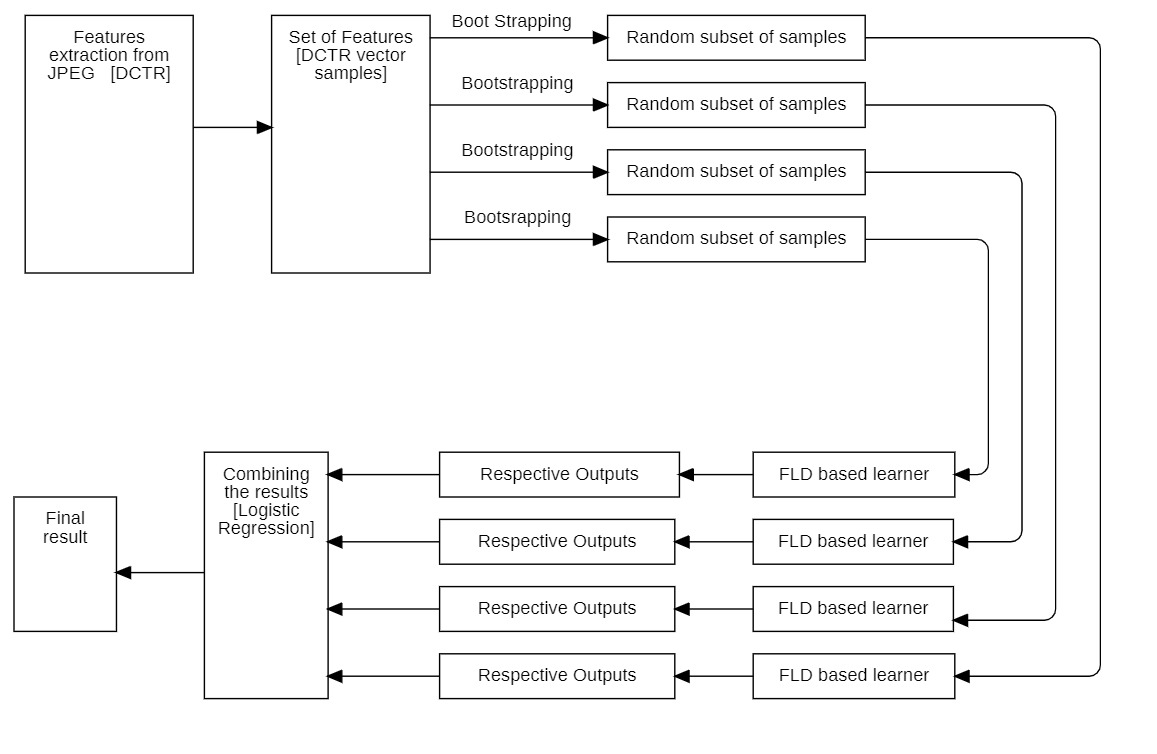
\includegraphics[width=1.1\textwidth]{./img/block_d.jpg} \\
\caption{ Block diagram of proposed system}
\end{figure}
\section{Description of working flow of proposed system}
this is data flow



